% Provenance (never printed): see sources/outline_sources.md (Year 3:
% critical-taper theory; fold-and-thrust belts; exhumation and
% thermochronology). Brief: sources/book5/BRIEFS.md, ch. 10. Curves from
% figdata/bachelor-3/fault_bend.py, critical_taper.py and age_elevation.py.
% Exercise and problem values in the Book 5 scratch calculator calc/ch10.py.
\chapter{Cinturões de cavalgamento e cunhas orogênicas}\label{ch:b3:orogenic-wedges}

Ao empurrar um trator de lâmina contra areia úmida ou neve, uma cunha de material se acumula
à frente da lâmina. Ela se deforma até que sua superfície atinja certa inclinação;
daí em diante desliza para a frente como um todo e cresce mantendo a mesma forma,
incorporando material novo na sua extremidade frontal. As partes externas dos cinturões de montanhas, desde
Taiwan até os sopés dos Alpes, comportam-se do mesmo modo: são cunhas de rocha
raspadas de uma placa e empurradas sobre uma base fraca, e a inclinação de sua superfície
e o mergulho da base indicam quão fraca ela é e quão alta é a
pressão dos fluidos que ela contém. Este capítulo constrói a geometria dos
cinturões de cavalgamento, a mecânica da cunha e os relógios que medem a rapidez com que suas
rochas chegam à superfície.
% ledger: dsd83:taper

\begin{recall}
Cavalgamentos, vergência e geometria de dobras estão no volume do primeiro ano, no capítulo
sobre falhas, dobras e tramas; o critério de Coulomb, a lei de Byerlee, a
tensão efetiva e a razão de pressão de poro $\lambda = P/\sigma_v$ no seu
capítulo sobre tensão, deformação e reologia; a temperatura de fechamento e a idade de resfriamento
no capítulo sobre métodos de datação radiométrica. O descolamento, a
cinturão de dobras e cavalgamentos, tectônica de pele fina e de pele grossa e a seção balanceada
estão no volume do segundo ano, no capítulo sobre a anatomia de um
cinturão de montanhas; a exumação e sua taxa estão no capítulo sobre trajetórias P--T--t. A
construção de kink e a área em excesso $A = Sh$ de uma dobra acima de um descolamento
estão no \cref{ch:b3:structural-analysis}; o \omterm{def:b3:lithosphere-thermal-models:peclet}{número de Péclet térmico} está
no \cref{ch:b3:lithosphere-thermal-models}.
\end{recall}

\section{A geometria dos cavalgamentos}\label{sec:b3:orogenic-wedges:geometry}

Um cavalgamento não corta uma sequência estratificada ao longo de um único plano reto.
Ele segue uma camada fraca, um folhelho ou um evaporito, por longas distâncias, e depois
sobe abruptamente pelas camadas resistentes acima até a próxima camada fraca. A
escada que ele desenha controla as dobras do bloco superior.

\begin{definition}[Rampa, patamar, duplex, cavalgamento fora de sequência]\label{def:b3:orogenic-wedges:thrust-geometry}
Um \emph{patamar (de cavalgamento)}\index{patamar (de cavalgamento)} é um segmento de cavalgamento que corre
paralelo ao acamamento, geralmente em uma camada fraca; uma \emph{rampa
(de cavalgamento)}\index{rampa (de cavalgamento)} é um segmento que corta o acamamento,
tipicamente de 20 a \ang{30}, unindo um patamar inferior a um superior. Um
\emph{duplex (de cavalgamento)}\index{duplex (de cavalgamento)} é uma pilha de fatias limitadas por falhas,
fatias, os \textit{horses}, confinadas entre um cavalgamento de base abaixo e um de teto
acima, cada \textit{horse} limitada por uma rampa que une os dois. Cavalgamentos costumam se formar
em sequência, cada novo cavalgamento no bloco inferior do anterior, mais próximo do
antepaís; um \emph{cavalgamento fora de sequência}\index{cavalgamento fora de sequência} é
um que se forma ou volta a deslizar atrás da frente ativa, cortando cavalgamentos mais antigos.
\end{definition}

À medida que o bloco superior se desloca sobre uma curvatura da falha, ele precisa se dobrar para permanecer em
contato com ela: um sinclinal se forma onde ele entra na rampa e um anticlinal
onde ele sai da rampa.

\begin{definition}[Dobras de curvatura de falha, de propagação de falha e de descolamento]\label{def:b3:orogenic-wedges:thrust-folds}
Uma \emph{dobra de curvatura de falha}\index{dobra de curvatura de falha} é uma dobra do bloco superior
de um cavalgamento, formada à medida que ele desliza sobre uma curvatura da falha, uma rampa entre
dois patamares. Uma \emph{dobra de propagação de falha}\index{dobra de propagação de falha}
cresce acima da ponta de um cavalgamento que ainda se propaga para cima: o
encurtamento que a falha já não transporta é absorvido por dobramento à frente
de sua ponta, o que resulta em um flanco frontal íngreme ou invertido. Uma \emph{dobra de
descolamento}\index{dobra de descolamento} cresce acima de um patamar sem rampa: o encurtamento
é absorvido por dobramento e por uma camada fraca, de sal ou folhelho, que flui para
seu núcleo.
\end{definition}

A figura abaixo constrói uma \omterm{def:b3:orogenic-wedges:thrust-folds}{dobra de curvatura de falha}. Aqui o bloco superior se move
paralelamente ao segmento de falha abaixo dele e se dobra em superfícies axiais que
bissectam cada curvatura, um modelo cinemático chamado fluxo paralelo à falha; o clássico
modelo de espessura e comprimento de camadas constantes produz o mesmo
anticlinal de topo plano, com um flanco frontal mais íngreme, ao custo de uma construção mais longa
(aqui admitida). Ambos os modelos são limitados pela conservação de área.

\begin{omfigure}
\begin{tikzpicture}
\begin{groupplot}[group style={group size=1 by 2, vertical sep=0.9cm},
  width=0.92\linewidth, axis equal image,
  xmin=0, xmax=12, ymin=-0.6, axis lines=none, clip=true,
  title style={font=\small, at={(0.0,1.0)}, anchor=south west}]
% (a) before slip
\nextgroupplot[title={(a) antes do deslizamento}, ymax=1.75]
\fill[omLithSand!70] (axis cs:0,0) rectangle (axis cs:12,1.6);
\fill[gray!25] (axis cs:0,-0.6) rectangle (axis cs:12,0);
\draw[black!70] (axis cs:0,0.25) -- (axis cs:12,0.25);
\draw[black!70] (axis cs:0,0.5) -- (axis cs:12,0.5);
\draw[black!70] (axis cs:0,0.75) -- (axis cs:12,0.75);
\draw[black!70] (axis cs:0,1.0) -- (axis cs:12,1.0);
\draw[black!70] (axis cs:0,1.3) -- (axis cs:12,1.3);
\draw[black!70] (axis cs:0,1.6) -- (axis cs:12,1.6);
\draw[black!70] (axis cs:0,-0.3) -- (axis cs:12,-0.3);
\addplot[very thick, red!70!black] table[x=x, y=y] {figdata/out/bachelor-3-fault_bend-fault.dat};
\node[font=\scriptsize, fill=omLithSand!70, inner sep=1pt] at (axis cs:2,0.125) {patamar inferior};
\node[font=\scriptsize, fill=omLithSand!70, inner sep=1pt, rotate=30] at (axis cs:4.55,0.62) {rampa};
\node[font=\scriptsize, fill=omLithSand!70, inner sep=1pt] at (axis cs:9,0.875) {patamar superior};
% (b) after a slip of 2.5 units
\nextgroupplot[title={(b) após o deslizamento: uma dobra de curvatura de falha}, ymax=2.75]
\fill[gray!25] (axis cs:0,-0.6) rectangle (axis cs:12,0) -- cycle;
\addplot[name path=fault, draw=none] table[x=x, y=y] {figdata/out/bachelor-3-fault_bend-fault.dat};
\addplot[name path=top, draw=none] table[x=x, y=y] {figdata/out/bachelor-3-fault_bend-bed6.dat};
\addplot[name path=base, draw=none] coordinates {(0,-0.6) (12,-0.6)};
\addplot[omLithSand!70] fill between[of=fault and top];
\addplot[gray!25] fill between[of=base and fault];
\addplot[black!70] table[x=x, y=y] {figdata/out/bachelor-3-fault_bend-bed1.dat};
\addplot[black!70] table[x=x, y=y] {figdata/out/bachelor-3-fault_bend-bed2.dat};
\addplot[black!70] table[x=x, y=y] {figdata/out/bachelor-3-fault_bend-bed3.dat};
\addplot[black!70] table[x=x, y=y] {figdata/out/bachelor-3-fault_bend-bed4.dat};
\addplot[black!70] table[x=x, y=y] {figdata/out/bachelor-3-fault_bend-bed5.dat};
\addplot[black!70] table[x=x, y=y] {figdata/out/bachelor-3-fault_bend-bed6.dat};
\draw[black!70] (axis cs:4.4330,0.25) -- (axis cs:12,0.25);
\draw[black!70] (axis cs:4.8660,0.5) -- (axis cs:12,0.5);
\draw[black!70] (axis cs:5.2990,0.75) -- (axis cs:12,0.75);
\draw[black!70] (axis cs:0,-0.3) -- (axis cs:12,-0.3);
\addplot[very thick, red!70!black] table[x=x, y=y] {figdata/out/bachelor-3-fault_bend-fault.dat};
\draw[densely dashed, black!60] (axis cs:0,1.6) -- (axis cs:12,1.6);
\node[font=\scriptsize, anchor=south] at (axis cs:2.2,1.65) {regional};
\node[font=\scriptsize, anchor=west] at (axis cs:8.6,2.25) {área em excesso $A = Sr$};
\draw[black!70] (axis cs:8.6,2.25) -- (axis cs:6.6,2.0);
\node[font=\scriptsize, fill=gray!25, inner sep=1pt] at (axis cs:10.6,0.625) {bloco inferior};
\end{groupplot}
\end{tikzpicture}

\par\smallskip{\small (a) Um cavalgamento com um patamar inferior, uma rampa com mergulho de
\ang{30} e um patamar superior, antes do deslocamento (esquemático, com escalas vertical e horizontal
iguais). (b) O mesmo após um deslocamento de 2.5 vezes a altura da rampa,
calculado por fluxo paralelo à falha: um sinclinal no sopé da rampa, um flanco posterior
paralelo à rampa, uma crista plana erguida pela altura da rampa $r$, um
flanco frontal e uma área em excesso $Sr$ acima do nível regional de cada camada acima
do patamar superior.}\label{fig:b3:orogenic-wedges:thrusts}
\end{omfigure}


\begin{proposition}[Área em excesso de uma dobra de curvatura de falha]\label{prop:b3:orogenic-wedges:fault-bend-area}
Suponha-se que uma falha de cavalgamento eleve seu bloco superior por uma rampa de altura $r$, partindo de um patamar inferior
até um patamar superior, com o deslocamento $S$ sobre o patamar inferior. Para qualquer camada do
bloco superior que esteja acima do patamar superior, a área delimitada entre a camada dobrada e o
seu nível original é $A = Sr$, a mesma para toda camada desse tipo.
\end{proposition}

\begin{proof}
Considere-se que a rocha não é criada nem destruída, e seu volume é conservado. Considere-se uma seção
paralela ao deslocamento, delimitada por duas linhas verticais, uma bem atrás e outra bem
à frente da rampa. Pela linha traseira, o bloco superior entre o patamar inferior e uma camada
à altura $y_0$ acima dele avançou $S$ para dentro: entrou a área
$Sy_0$. Pela linha frontal, a rocha entre o patamar superior e a
mesma camada, de espessura $y_0 - r$, saiu pelo deslocamento sobre o
patamar superior, também $S$ quando a rocha conserva sua área: a área $S(y_0 - r)$
saiu. A diferença, $Sr$, ficou entre as duas linhas e eleva
a camada acima de seu nível original.
\end{proof}

A área em excesso de uma \omterm{def:b3:orogenic-wedges:thrust-folds}{dobra de curvatura de falha} mede o deslocamento vezes a altura da
rampa, e não vezes a profundidade do descolamento, como ocorreria para uma
\omterm{def:b3:orogenic-wedges:thrust-folds}{dobra de descolamento} (no \cref{ch:b3:structural-analysis}). Os dois tipos de dobra
devem ser distinguidos antes que uma área seja convertida em encurtamento.


Um duplex (figura abaixo) cresce quando o cavalgamento, em vez de levar seu bloco superior cada vez mais
adiante ao longo da mesma rampa, a abandona e corta uma nova rampa em seu bloco inferior,
à frente da antiga. A fatia entre a rampa antiga e a nova torna-se um
cavalo, levado pela nova rampa acima e empilhado sob o teto; a próxima rampa
forma-se de novo à frente. Cada cavalo sofre encurtamento de seu comprimento original até o
comprimento que ocupa agora ao longo da base, e o encurtamento do duplex é
a soma sobre seus cavalos. \omterm{def:b3:orogenic-wedges:thrust-geometry}{Cavalgamentos fora de sequência} quebram essa ordem: formam-se
quando a cunha atrás da frente precisa engrossar, caso que a mecânica da
próxima seção prevê.

\begin{omfigure}
\begin{tikzpicture}
\begin{axis}[width=0.92\linewidth, axis equal image, xmin=0, xmax=12, ymin=-0.6, ymax=1.95,
  axis lines=none, clip=true]
\fill[gray!25] (axis cs:0,-0.6) rectangle (axis cs:12,0);
\fill[omLithSand!70] (axis cs:0,0) -- (axis cs:1.0,0) -- (axis cs:2.35,1.15) -- (axis cs:12,1.15) -- (axis cs:12,1.85) -- (axis cs:2.35,1.85) -- (axis cs:1.0,0.7) -- (axis cs:0,0.7) -- cycle;
\draw[black!70] (axis cs:0,0.35) -- (axis cs:1.0,0.35) -- (axis cs:2.35,1.5) -- (axis cs:12,1.5);
\draw[black!70] (axis cs:0,0.7) -- (axis cs:1.0,0.7) -- (axis cs:2.35,1.85) -- (axis cs:12,1.85);
\fill[omLithShale!60] (axis cs:8.2,0) -- (axis cs:12,0) -- (axis cs:12,1.15) -- (axis cs:9.55,1.15) -- cycle;
\draw[black!70] (axis cs:8.646,0.38) -- (axis cs:12,0.38);
\draw[black!70] (axis cs:9.104,0.77) -- (axis cs:12,0.77);
\fill[omLithLime] (axis cs:1.0,0) -- (axis cs:2.80,0) -- (axis cs:4.15,1.15) -- (axis cs:2.35,1.15) -- cycle;
\draw[black!70] (axis cs:1.45,0) -- (axis cs:2.80,1.15);
\draw[black!70] (axis cs:1.90,0) -- (axis cs:3.25,1.15);
\draw[black!70] (axis cs:2.35,0) -- (axis cs:3.70,1.15);
\fill[omLithShale] (axis cs:2.8,0) -- (axis cs:4.60,0) -- (axis cs:5.95,1.15) -- (axis cs:4.15,1.15) -- cycle;
\draw[black!70] (axis cs:3.25,0) -- (axis cs:4.60,1.15);
\draw[black!70] (axis cs:3.70,0) -- (axis cs:5.05,1.15);
\draw[black!70] (axis cs:4.15,0) -- (axis cs:5.50,1.15);
\fill[omLithLime] (axis cs:4.6,0) -- (axis cs:6.40,0) -- (axis cs:7.75,1.15) -- (axis cs:5.95,1.15) -- cycle;
\draw[black!70] (axis cs:5.05,0) -- (axis cs:6.40,1.15);
\draw[black!70] (axis cs:5.50,0) -- (axis cs:6.85,1.15);
\draw[black!70] (axis cs:5.95,0) -- (axis cs:7.30,1.15);
\fill[omLithShale] (axis cs:6.4,0) -- (axis cs:8.20,0) -- (axis cs:9.55,1.15) -- (axis cs:7.75,1.15) -- cycle;
\draw[black!70] (axis cs:6.85,0) -- (axis cs:8.20,1.15);
\draw[black!70] (axis cs:7.30,0) -- (axis cs:8.65,1.15);
\draw[black!70] (axis cs:7.75,0) -- (axis cs:9.10,1.15);
\draw[thick, red!70!black] (axis cs:1.0,0) -- (axis cs:2.35,1.15);
\draw[thick, red!70!black] (axis cs:2.8,0) -- (axis cs:4.15,1.15);
\draw[thick, red!70!black] (axis cs:4.6,0) -- (axis cs:5.95,1.15);
\draw[thick, red!70!black] (axis cs:6.4,0) -- (axis cs:7.75,1.15);
\draw[thick, red!70!black] (axis cs:8.2,0) -- (axis cs:9.55,1.15);
\draw[very thick, red!70!black] (axis cs:0,0) -- (axis cs:12,0);
\draw[very thick, red!70!black] (axis cs:2.35,1.15) -- (axis cs:12,1.15);
\node[font=\scriptsize, anchor=north west] at (axis cs:0.1,-0.04) {cavalgamento de base};
\node[font=\scriptsize, anchor=south west] at (axis cs:7.0,1.17) {cavalgamento de teto};
\node[font=\scriptsize, anchor=north] at (axis cs:5.6,-0.12) {cavalo};
\draw[black!70] (axis cs:5.6,-0.15) -- (axis cs:5.5,0.45);
\draw[->, thick] (axis cs:0.15,0.52) -- (axis cs:0.95,0.52);
\end{axis}
\end{tikzpicture}

\par\smallskip{\small Um duplex (esquemático): quatro cavalos (azul e verde) cortados
por rampas entre um cavalgamento de base e um cavalgamento de teto, à frente deles o bloco inferior ainda não
cortado, a seta indicando o sentido do transporte; a cobertura acima do teto é
dobrada sobre a pilha.}\label{fig:b3:orogenic-wedges:duplex}
\end{omfigure}


\section{O afilamento crítico}\label{sec:b3:orogenic-wedges:taper}

Um cinturão de dobras e cavalgamentos, em seção transversal, é uma cunha: fina em sua frente, onde
o descolamento atinge a superfície, e engrossando em direção ao interior do orógeno.
Sua superfície superior inclina-se em direção ao antepaís com o ângulo $\alpha$; sua
base, o descolamento, mergulha em direção ao interior do orógeno com o ângulo $\beta$. O
afilamento da cunha é o ângulo entre elas, $\alpha + \beta$.

\begin{definition}[Afilamento crítico]\label{def:b3:orogenic-wedges:critical-taper}
O \emph{afilamento crítico}\index{afilamento crítico} de uma cunha empurrada por trás
sobre uma base é o afilamento em que a cunha está, em toda parte, na iminência de
ruptura, no interior e ao longo de sua base, sob compressão horizontal. Uma cunha no
afilamento crítico desliza sobre sua base sem se deformar internamente; uma
cunha abaixo dele (subcrítica) deforma-se e engrossa até atingi-lo; uma
cunha acima dele (supercrítica) desliza sem se deformar.
\end{definition}
% ledger: dsd83:taper

\begin{omfigure}
\begin{tikzpicture}[>=stealth, x=1cm, y=1cm]
\fill[omLithSand!70] (0,0) -- (10,-1.05) -- (10,1.4) -- cycle;
\fill[gray!25] (0,0) -- (10,-1.05) -- (10,-1.6) -- (-0.8,-1.6) -- (-0.8,0) -- cycle;
\draw[thick] (-0.8,0) -- (0,0) -- (10,1.4);
\draw[very thick, red!70!black] (0,0) -- (10,-1.05);
\fill[gray!60] (10,-1.6) rectangle (10.6,1.9);
\node[font=\scriptsize, rotate=90] at (10.3,0.15) {anteparo};
\draw[dashed] (0,0) -- (2.6,0);
\draw (2.2,0) arc[start angle=0, end angle=8, radius=2.2];
\node[font=\small] at (2.45,0.2) {$\alpha$};
\draw (2.2,0) arc[start angle=0, end angle=-6, radius=2.2];
\node[font=\small] at (2.45,-0.2) {$\beta$};
% slice
\draw[thick, omDef] (5.5,-0.5775) -- (5.5,0.77);
\draw[thick, omDef] (6.5,-0.6825) -- (6.5,0.91);
\draw[->, thick, omDef] (4.5,0.05) -- (5.45,0.05);
\node[font=\scriptsize, anchor=east] at (4.5,0.05) {$F(x)$};
\draw[<-, thick, omDef] (6.55,0.1) -- (7.6,0.1);
\node[font=\scriptsize, anchor=west] at (7.6,0.1) {$F(x + \mathrm dx)$};
\draw[->, thick, omProp] (6.0,-0.63) -- (6.75,-0.71);
\node[font=\scriptsize, anchor=north] at (6.4,-0.75) {$\tau_b$};
\draw[->, thick, omProp] (6.0,-0.63) -- (6.1,0.0);
\node[font=\scriptsize, anchor=east] at (6.02,-0.22) {$\sigma_n$};
\node[font=\scriptsize] at (6.0,1.2) {fatia $\mathrm dx$};
\draw[->, thick] (1.8,-1.25) -- (0.6,-1.25);
\node[font=\scriptsize, anchor=west] at (1.85,-1.25) {transporte};
\node[font=\scriptsize, anchor=west] at (0.2,-0.42) {descolamento};
\node[font=\scriptsize] at (8.9,-0.45) {cunha};
\draw[->] (0.1,0.5) -- (0.4,0.5); \node[font=\scriptsize, anchor=east] at (0.1,0.5) {$x$};
\end{tikzpicture}

\par\smallskip{\small Uma cunha de declividade superficial $\alpha$ apoiada sobre um
descolamento de mergulho $\beta$ e empurrada por trás; $x$ é medido a partir da
ponta em direção ao retroterra. Em uma fatia vertical, o empuxo $F(x + \mathrm dx)$
por trás excede o empuxo $F(x)$ da frente pelo que a base absorve:
seu atrito $\tau_b$ e a parte horizontal de sua tensão normal $\sigma_n$,
que se inclina em direção ao retroterra, em uma base que mergulha nesse sentido (esquemático,
ângulos exagerados).}\label{fig:b3:orogenic-wedges:wedge}
\end{omfigure}

\begin{theorem}[Equação do afilamento crítico]\label{thm:b3:orogenic-wedges:critical-taper}
Considera-se uma cunha subaérea de densidade uniforme $\rho$ constituída de material de Coulomb sem coesão
de atrito interno $\mu = \tan\phi$, com a razão de pressão de poros
$\lambda$, sobre uma base de atrito $\mu_b$ e razão de pressão de poros
$\lambda_b$. Se $\alpha$ e $\beta$ são pequenos e $\sigma_1$ é horizontal,
a \emph{equação do afilamento crítico}\index{equação do afilamento crítico} é
\[
  \alpha + \beta = \frac{\beta + \mu_b(1 - \lambda_b)}{1 + K(1 - \lambda)},
  \qquad K = \frac{2\sin\phi}{1 - \sin\phi},
\]
com os ângulos em radianos.
\end{theorem}

\begin{proof}
Seja $z$ a profundidade abaixo da superfície. Com declividades pequenas, a tensão vertical
é o peso da rocha sobrejacente, $\sigma_{zz} = \rho g z$, e a pressão de poros
é $\lambda\rho g z$, de modo que a tensão vertical efetiva é
$(1 - \lambda)\rho g z$. Em toda parte na ruptura, com $\sigma_1$ horizontal,
o critério de Coulomb para material sem coesão fornece a razão entre as
tensões principais efetivas $\sigma'_1/\sigma'_3 = (1 + \sin\phi)/(1 -
\sin\phi) = 1 + K$, logo a tensão horizontal total
\[
  \sigma_{xx} = (1 + K)(1 - \lambda)\rho g z + \lambda\rho g z
  = \bigl(1 + K(1 - \lambda)\bigr)\rho g z .
\]
A uma distância $x$ da ponta, a cunha tem espessura $H = (\alpha +
\beta)x$, e a força horizontal por unidade de comprimento do cinturão em uma seção vertical
é $F = \int_0^H \sigma_{xx}\,\mathrm dz = \bigl(1 + K(1 -
\lambda)\bigr)\rho g H^2/2$. Na fatia entre $x$ e $x + \mathrm dx$
(a figura acima), a superfície não suporta tensão e o empuxo por trás
excede o empuxo da frente em $(\mathrm dF/\mathrm dx)\,\mathrm dx$.
A base retém a fatia de duas maneiras: pelo atrito $\mu_b(1 -
\lambda_b)\rho g H$ por unidade de comprimento, e pela sua tensão normal $\rho g H$, que
é perpendicular a uma base que mergulha $\beta$ em direção ao retroterra e, por isso,
inclina-se nesse sentido de $\beta$, resultando na parte horizontal $\beta\rho g H$.
O equilíbrio da fatia exige
\[
  \bigl(1 + K(1 - \lambda)\bigr)\rho g H(\alpha + \beta)
  = \bigl(\beta + \mu_b(1 - \lambda_b)\bigr)\rho g H ,
\]
que é a equação. Como $H$ se cancela, uma cunha na ruptura mantém o mesmo
afilamento à medida que cresce.
\end{proof}

A equação mostra, em primeiro lugar, que o afilamento é fixado pela razão entre a resistência
da base, no numerador, e a resistência da cunha, no
denominador: uma base fraca produz uma cunha delgada, uma base forte, uma cunha espessa.
Em segundo lugar, a declividade superficial diminui à medida que a base mergulha mais acentuadamente. Em terceiro lugar, a pressão do fluido
reduz o afilamento: elevar $\lambda = \lambda_b$ retira da
resistência da base, proporcionalmente, mais do que da resistência da
cunha. A figura abaixo mostra a declividade superficial crítica para os coeficientes de atrito
ajustados no oeste de Taiwan. Os pontos abaixo de cada linha são cunhas subcríticas,
que se espessam; os pontos acima são supercríticos, que deslizam.
% ledger: dsd83:taper

\begin{omfigure}
\begin{tikzpicture}
\begin{axis}[omrecord, width=0.8\linewidth, height=0.5\linewidth,
  xlabel={mergulho basal $\beta$ (\unit{\degree})}, ylabel={declividade superficial $\alpha$ (\unit{\degree})},
  xmin=0, xmax=15, ymin=0, ymax=12, legend style={font=\scriptsize, at={(0.98,0.98)},
  anchor=north east, legend cell align=left}]
% computed in figdata/bachelor-3/critical_taper.py
\addplot[name path=t3, draw=none, forget plot] table[x=beta, y=t3] {figdata/out/bachelor-3-critical_taper-bands.dat};
\addplot[name path=t4, draw=none, forget plot] table[x=beta, y=t4] {figdata/out/bachelor-3-critical_taper-bands.dat};
\addplot[name path=t12, draw=none, forget plot] table[x=beta, y=t12] {figdata/out/bachelor-3-critical_taper-bands.dat};
\addplot[name path=t13, draw=none, forget plot] table[x=beta, y=t13] {figdata/out/bachelor-3-critical_taper-bands.dat};
\addplot[omLithEvap, area legend] fill between[of=t3 and t4];
\addlegendentry{afilamento 3--\ang{4} (Jura)}
\addplot[omLithLime, area legend] fill between[of=t12 and t13];
\addlegendentry{afilamento 12--\ang{13}}
\addplot[omDef, thick] table[x=beta, y=a040] {figdata/out/bachelor-3-critical_taper-curves.dat};
\addlegendentry{$\lambda = 0.4$}
\addplot[red!70!black, thick, densely dashed] table[x=beta, y=a070] {figdata/out/bachelor-3-critical_taper-curves.dat};
\addlegendentry{$\lambda = 0.7$}
\addplot[black, thick, densely dotted] table[x=beta, y=a090] {figdata/out/bachelor-3-critical_taper-curves.dat};
\addlegendentry{$\lambda = 0.9$}
\node[font=\scriptsize] at (axis cs:2.2,1.1) {subcrítico};
\node[font=\scriptsize] at (axis cs:1.6,8.6) {supercrítico};
\end{axis}
\end{tikzpicture}

\par\smallskip{\small Inclinação crítica da superfície em função do mergulho basal para os
coeficientes de atrito do oeste de Taiwan, $\mu = 1.03$ no interior e $\mu_b =
0.85$ na base, para três razões de pressão de poros $\lambda = \lambda_b$;
``subcrítico'' e ``supercrítico'' referem-se à linha $\lambda = 0.7$. As
faixas sombreadas são os afilamentos da cunha de cavalgamento do Jura, de 3 a \ang{4}, e da
cunha ao sul dela, de 12 a \ang{13}.}\label{fig:b3:orogenic-wedges:taper}
\end{omfigure}
% ledger: dsd83:taper, deville21:jura

Uma cunha não é um objeto estático: material é acrescentado a ela e removido dela,
e cada mudança a desloca de seu \omterm{def:b3:orogenic-wedges:critical-taper}{afilamento crítico}.

\begin{definition}[Acreção frontal, underplating tectônico]\label{def:b3:orogenic-wedges:accretion}
A \emph{acreção frontal}\index{acreção frontal} é a adição de material
a uma cunha em sua ponta, à medida que o descolamento se propaga para dentro dos
sedimentos não deformados do antepaís e uma nova lasca de cavalgamento é cortada. O \emph{underplating
tectônico}\index{underplating tectônico} é a adição de material à
base da cunha, atrás de sua ponta, à medida que lascas da placa inferior são
destacadas e empilhadas sob ela, com frequência na forma de duplexes.
\end{definition}

A \omterm{def:b3:orogenic-wedges:accretion}{acreção frontal} alonga a cunha mantendo o afilamento constante. O underplating
espessa sua retaguarda e torna sua superfície mais íngreme: a cunha torna-se supercrítica
ali e pode se estender por falhamento normal até que o afilamento volte a diminuir. A erosão
faz o oposto: rebaixa a inclinação da superfície, a cunha torna-se
subcrítica e se espessa por \omterm{def:b3:orogenic-wedges:thrust-geometry}{cavalgamento fora de sequência} atrás da frente.
Erosão e deformação estão, assim, acopladas: uma cunha erodida rapidamente mantém seu
afilamento movendo a rocha para cima mais depressa, e as rochas que ela traz à superfície
são mais jovens no sentido da próxima seção.

\begin{inthelab}[Modelos em caixa de areia]
\begin{minipage}[t]{0.55\linewidth}\vspace{0pt}
Em um modelo analógico de caixa de areia, camadas de areia seca de cores diferentes são
depositadas horizontalmente em uma caixa longa de vidro. Um motor empurra lentamente uma parede vertical contra elas,
ou puxa uma folha de sob elas; uma câmera ao lado do vidro fotografa a seção em intervalos
regulares. A areia rompe ao longo de cavalgamentos, forma uma cunha que mantém um
afilamento constante e desenvolve rampas, duplexes e cavalgamentos de retorno semelhantes aos de
cinturões reais. Uma camada de esferas de vidro ou de massa de silicone sob a areia faz o papel
de um descolamento fraco, e a cunha então cresce mais fina e mais larga.
Davis, Suppe e Dahlen constataram que seus experimentos com areia seca concordavam com a
teoria do \omterm{def:b3:orogenic-wedges:critical-taper}{afilamento crítico}. A correlação das fotografias sucessivas fornece o
campo de deslocamentos no interior do modelo.
\end{minipage}\hfill
\begin{minipage}[t]{0.42\linewidth}\vspace{0pt}
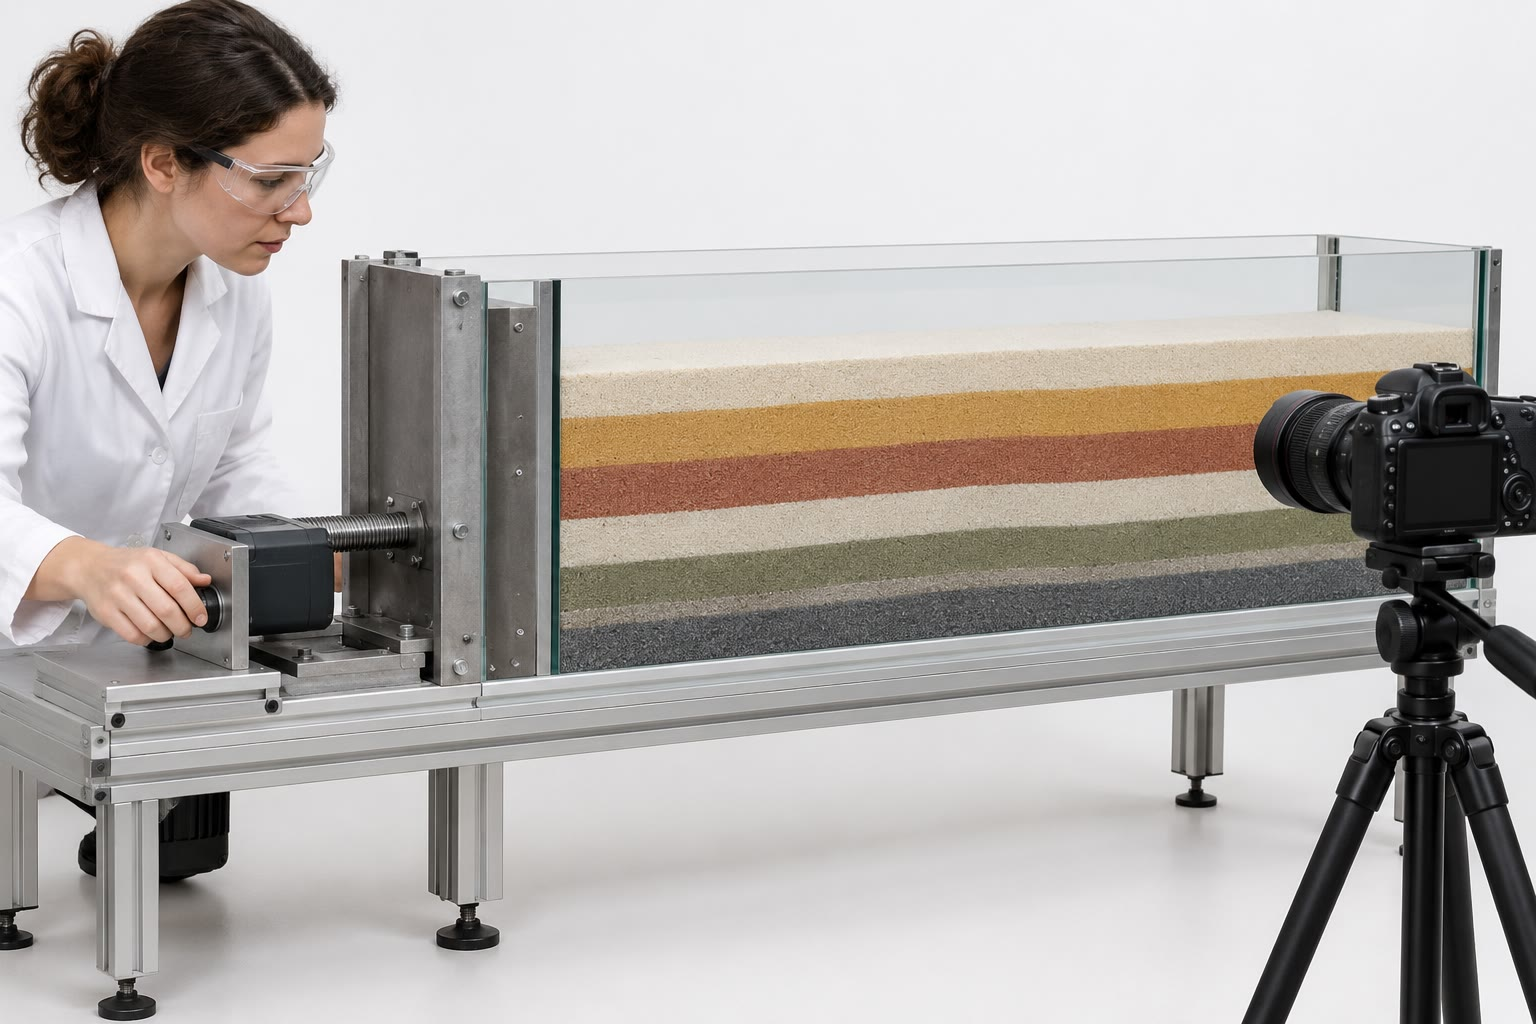
\includegraphics[width=\linewidth]{images/book5/ai/b3-sandbox-lab.jpg}

{\scriptsize Um modelo de caixa de areia antes do encurtamento: camadas de areia colorida em uma
caixa de vidro, uma parede acionada por motor à esquerda, uma câmera sobre um tripé
(Ilustração gerada por IA.)}
\end{minipage}
\end{inthelab}
% ledger: dsd83:taper

\section{Cunhas reais}\label{sec:b3:orogenic-wedges:real}

No cinturão ativo de dobramentos e cavalgamentos do oeste de Taiwan, a inclinação da superfície, o
mergulho do descolamento e as pressões de poros são todos conhecidos, a partir da topografia,
de seções sísmicas e de poços. Davis, Suppe e Dahlen os utilizaram para resolver a
\omterm{thm:b3:orogenic-wedges:critical-taper}{equação do afilamento crítico} quanto à resistência da cunha e obtiveram $\mu = 1.03$
no interior e $\mu_b = 0.85$ na base: o atrito de Byerlee na base, e uma
cunha mais resistente do que suas próprias falhas, porque nem todas estão orientadas para deslizar
com facilidade. Com esses dois coeficientes, converteram os afilamentos observados de outras
cunhas ativas, em terra e sob o mar, em razões de pressão de poros, e as encontraram
sempre acima da hidrostática, em concordância com as perfurações. Também constataram
onde a teoria deixa de valer: o afilamento cai abruptamente onde as cunhas se tornam mais espessas
do que cerca de \qty{15}{km}, a profundidade em que rochas ricas em quartzo se tornam plásticas
para geotermas comuns, e a base deixa de obedecer a uma lei friccional.
% ledger: dsd83:taper

No front dos Alpes ocidentais, o Jura é uma cunha de cavalgamento com ângulo estreito
de apenas 3 a \ang{4}. Seu descolamento situa-se sobretudo em camadas com halita
de idade triássica, e os fluidos ali não estão sobrepressurizados: a
fraqueza do sal, por si só, explica o afilamento estreito. Ao sul do Jura, onde as
camadas triássicas não contêm halita, a mesma frente apresenta um afilamento de 12 a
\ang{13}, com pilhas de lascas de cavalgamento, embora as pressões de fluido ali medidas
sejam altas. Nos Alpes Centrais, a análise do \omterm{def:b3:orogenic-wedges:critical-taper}{afilamento crítico}, com base na
inclinação da superfície, fornece uma resistência basal $\mu_b(1 - \lambda_b)$ (com um pequeno termo de
coesão) abaixo de 0.1, e até 0.05 em evaporitos e folhelhos próximos à frente,
aumentando em direção ao hinterlândia, com razões de pressão de poros acima de 0.54. A
base de uma cunha é muitas vezes muito mais fraca do que a lei de Byerlee faria supor, por causa de seu
tipo de rocha e de seus fluidos.
% ledger: deville21:jura, vonhagke14:alps

\section{Fluxo através de uma cunha}\label{sec:b3:orogenic-wedges:flux}

Uma cunha em seu \omterm{def:b3:orogenic-wedges:critical-taper}{afilamento crítico} cresce por acreção, com forma fixa: seu comprimento
e sua altura aumentam juntos. A erosão remove rocha de sua superfície. Quando as
duas se equilibram, a cunha mantém seu tamanho, e a rocha flui através dela.

\begin{proposition}[Balanço de fluxo em estado estacionário]\label{prop:b3:orogenic-wedges:flux}
Uma cunha de largura $W$ ao longo da direção de transporte recebe, por unidade de comprimento
do cinturão, o fluxo de acreção $F_a = v h$, onde $v$ é a taxa de convergência
e $h$ a espessura da camada incidente acima do descolamento. Ela
perde o fluxo erosivo $F_e = \bar e W$, onde $\bar e$ é a taxa média de erosão
sobre sua superfície. Sua área de seção transversal varia à taxa $F_a -
F_e$; em estado estacionário, $\bar e = vh/W$.
\end{proposition}

\begin{proof}
Em unidade de tempo, um comprimento $v$ da camada incidente, de espessura $h$, passa
para dentro da cunha através de sua ponta, e a espessura $e(x)$ é removida em cada
ponto de sua superfície; a área é conservada, de modo que a área da seção
varia de $vh - \int_0^W e\,\mathrm dx = F_a - F_e$. Em estado estacionário, a
variação é nula.
\end{proof}

Com $v = \qty{10}{mm/yr}$, $h = \qty{4}{km}$ e $W = \qty{60}{km}$, a
taxa de erosão necessária para o estado estacionário é $\qty{0.67}{mm/yr}$. A exumação, no
sentido do volume do segundo ano, é a remoção da rocha acima de uma dada rocha:
em estado estacionário, as rochas chegam à superfície na taxa em que a erosão rebaixa
a superfície, e a cunha as traz de profundidades onde eram quentes. Medir
a rapidez com que isso ocorre exige um relógio que comece a contar a partir de uma temperatura conhecida.

\section{Termocronologia}\label{sec:b3:orogenic-wedges:thermochronology}

\begin{definition}[Termocronologia, termocronômetro]\label{def:b3:orogenic-wedges:thermochronology}
A \emph{termocronologia}\index{termocronologia} é o uso de idades radiométricas
de resfriamento para datar o momento em que uma rocha passou por uma dada
temperatura e, assim, reconstruir sua história térmica. Um
\emph{termocronômetro}\index{termocronômetro} é o conjunto de um mineral e
de um método de datação, com sua temperatura de fechamento: por exemplo, apatita com o
método (U--Th)/He, ou zircão com traços de fissão.
\end{definition}

A tabela abaixo ordena os principais \omterm{def:b3:orogenic-wedges:thermochronology}{termocronômetros} pela temperatura de fechamento;
as profundidades pressupõem uma temperatura média na superfície de \qty{10}{\celsius} e uma
gradiente uniforme de \qty{30}{\celsius/km}. Uma rocha que se resfria à medida que é
exumada passa por eles em sequência, e suas idades aumentam dos métodos de baixa temperatura
para os de alta temperatura. A física dos traços de fissão e da
difusão de hélio, que fixa essas temperaturas, está no
\cref{ch:b3:advanced-geochronology}.
\begin{center}
\small
% ledger: sueoka19:closure
\begin{tabular}{lcc}
\hline
\omterm{def:b3:orogenic-wedges:thermochronology}{termocronômetro} & temperatura de fechamento (\unit{\celsius}) & profundidade (\unit{km}) \\
\hline
apatita (U--Th)/He & 50--80 & 1.3--2.3 \\
traço de fissão em apatita & 90--120 & 2.7--3.7 \\
zircão (U--Th)/He & 160--200 & 5.0--6.3 \\
traço de fissão em zircão & aproximadamente 280 & 9 \\
\textsuperscript{40}Ar/\textsuperscript{39}Ar em biotita & 350--400 & 11--13 \\
\textsuperscript{40}Ar/\textsuperscript{39}Ar em muscovita & aproximadamente 425 & 14 \\
U--Pb em zircão & acima de 900 & --- \\
\hline
\end{tabular}
\end{center}

Essas profundidades são apenas uma primeira estimativa, porque a erosão altera a geoterma.

\begin{proposition}[Geoterma em estado estacionário com erosão]\label{prop:b3:orogenic-wedges:geotherm}
Suponha-se que a rocha suba com velocidade constante $v$ através de uma camada de espessura $L$ cuja
superfície ($z = 0$) seja mantida em $T_s$ e a base em $T_L$, sem produção
interna de calor. A temperatura em regime estacionário é
\[
  T(z) = T_s + (T_L - T_s)\,\frac{1 - e^{-\mathrm{Pe}\,z/L}}{1 - e^{-\mathrm{Pe}}},
  \qquad \mathrm{Pe} = \frac{vL}{\kappa},
\]
e o gradiente na superfície é $\mathrm{Pe}/(1 - e^{-\mathrm{Pe}})$ vezes
o gradiente condutivo $(T_L - T_s)/L$.
\end{proposition}

\begin{proof}
Uma partícula de rocha na profundidade $z$ desloca-se para cima, em direção a valores menores de $z$: a
temperatura que ela carrega varia segundo $\partial T/\partial t - v\,\partial
T/\partial z$, e a equação de difusão torna-se $\partial T/\partial t - v
T' = \kappa T''$. Em regime estacionário, $T'' = -(v/\kappa)T'$, logo $T' = C
e^{-vz/\kappa}$ e $T = T_s + C(\kappa/v)(1 - e^{-vz/\kappa})$, o que satisfaz
$T(0) = T_s$. Impondo $T(L) = T_L$ fixa-se $C$ e obtém-se a fórmula. Em $z =
0$, $T' = (T_L - T_s)(\mathrm{Pe}/L)/(1 - e^{-\mathrm{Pe}})$.
\end{proof}

Para $\mathrm{Pe} \ll 1$, o fator tende a 1: a condução prevalece e a
geoterma permanece reta. Para $v = \qty{1}{mm/yr}$ ao longo de \qty{30}{km}, com
$\kappa = \qty{e-6}{m^2/s}$, $\mathrm{Pe} = 0.95$ e o gradiente na superfície
sobe de 30 para \qty{46}{\celsius/km}: as isotermas se concentram em direção à
superfície e cada \omterm{def:b3:orogenic-wedges:thermochronology}{termocronômetro} fecha-se a uma profundidade menor.
% ledger: england:kelvin, earle:settings

\begin{definition}[Relação idade--altitude]\label{def:b3:orogenic-wedges:age-elevation}
A \emph{relação idade--altitude}\index{relação idade--altitude} de um
\omterm{def:b3:orogenic-wedges:thermochronology}{termocronômetro} é o gráfico das idades de resfriamento de amostras coletadas em uma
faixa de altitudes, geralmente ao longo de uma encosta íngreme ou de um perfil vertical,
em função de suas altitudes.
\end{definition}

\begin{proposition}[Inclinação da relação idade--altitude]\label{prop:b3:orogenic-wedges:age-elevation}
Suponha-se que as rochas subam verticalmente com velocidade constante $v$ sob uma
topografia em regime estacionário, e que a isoterma de fechamento esteja na altitude $e(x) = e_0 +
f\,h(x)$, em que $h(x)$ é a altitude da superfície e $0 \le f < 1$. Uma amostra
coletada na superfície, na altitude $h$, tem idade $t = (h - e)/v$,
e a \omterm{def:b3:orogenic-wedges:age-elevation}{relação idade--altitude} é uma reta de inclinação
\[
  \frac{\mathrm dh}{\mathrm dt} = \frac{v}{1 - f}.
\]
Com isoterma plana, $f = 0$ e a inclinação é a taxa de exumação.
\end{proposition}

\begin{proof}
A rocha que agora está na superfície em $x$ cruzou a isoterma de fechamento logo abaixo,
na altitude $e(x)$, e desde então subiu $h - e$ à velocidade $v$:
$t = (h - e_0 - fh)/v = ((1 - f)h - e_0)/v$. Logo $\mathrm dt/\mathrm dh =
(1 - f)/v$.
\end{proof}

\begin{omfigure}
\begin{tikzpicture}
\begin{groupplot}[group style={group size=2 by 1, horizontal sep=1.7cm},
  omrecord, width=0.47\linewidth, height=0.45\linewidth, title style={font=\small},
  legend style={font=\scriptsize, legend cell align=left}]
\nextgroupplot[title={(a) idade--altitude}, xlabel={idade (U--Th)/He em apatita (\unit{Myr})},
  ylabel={altitude acima da média (\unit{km})}, xmode=log, xmin=0.1, xmax=10,
  log ticks with fixed point, xtick={0.1,0.2,0.5,1,2,5,10}, ymin=-1, ymax=1]
% computed in figdata/bachelor-3/age_elevation.py
\addplot[black, thick, densely dotted] table[x=a30, y=h] {figdata/out/bachelor-3-age_elevation-ages.dat};
\addplot[red!70!black, thick, densely dashed] table[x=a10, y=h] {figdata/out/bachelor-3-age_elevation-ages.dat};
\addplot[omDef, thick] table[x=a03, y=h] {figdata/out/bachelor-3-age_elevation-ages.dat};
\nextgroupplot[title={(b) isoterma de fechamento}, xlabel={distância (\unit{km})},
  ylabel={altitude acima da média (\unit{km})}, xmin=0, xmax=40, ymin=-3.3, ymax=1.2,
  legend style={at={(0.5,0.03)}, anchor=south, legend columns=2}]
\addplot[black!70, very thick] table[x=x, y=h] {figdata/out/bachelor-3-age_elevation-iso.dat};
\addlegendentry{superfície}
\addplot[black, thick, densely dotted] table[x=x, y=e30] {figdata/out/bachelor-3-age_elevation-iso.dat};
\addlegendentry{\qty{3}{mm/yr}}
\addplot[red!70!black, thick, densely dashed] table[x=x, y=e10] {figdata/out/bachelor-3-age_elevation-iso.dat};
\addlegendentry{\qty{1}{mm/yr}}
\addplot[omDef, thick] table[x=x, y=e03] {figdata/out/bachelor-3-age_elevation-iso.dat};
\addlegendentry{\qty{0.3}{mm/yr}}
\end{groupplot}
\end{tikzpicture}

\par\smallskip{\small Exumação estacionária sob um relevo senoidal de
comprimento de onda \qty{20}{km} e amplitude \qty{1}{km}, para três taxas,
estilos de linha como na legenda de (b) (modelo de primeira ordem; camada com \qty{30}{km} de espessura, superfície a \qty{10}{\celsius},
\qty{30}{\celsius/km} sem erosão, $\kappa = \qty{e-6}{m^2/s}$, taxa de
lapso \qty{6.5}{\celsius/km}, fechamento a \qty{65}{\celsius}). (a) Idade em função da
altitude: as inclinações são 0.59, 2.5 e \qty{14}{mm/yr}, e não 0.3, 1 e 3.
(b) A isoterma de \qty{65}{\celsius} acompanha a topografia tanto mais de perto
quanto mais rápida for a exumação, pois ela sobe mais perto da superfície.}\label{fig:b3:orogenic-wedges:age-elevation}
\end{omfigure}
% ledger: earle:settings, england:kelvin, ussa76:layers, sueoka19:closure

Isotermas não são planas sob um relevo: a superfície é mais fria nos picos
do que nos vales, pela taxa de lapso atmosférica, mas bem menos do que a rocha
estaria na mesma altitude em profundidade, e as isotermas rasas
acompanham a topografia de forma atenuada. Para uma topografia senoidal de
comprimento de onda $\Lambda$ e uma taxa de lapso $\Gamma$, uma solução de primeira ordem da
equação estacionária fornece
\[
  f = \frac{(G_0 - \Gamma)\,e^{-mz_c}}{G(z_c)},\qquad
  m = \frac{v}{2\kappa} + \sqrt{\Bigl(\frac{v}{2\kappa}\Bigr)^2 +
  \Bigl(\frac{2\pi}{\Lambda}\Bigr)^2},
\]
em que $z_c$ é a profundidade da isoterma de fechamento abaixo da superfície média,
$G_0$ o gradiente superficial e $G(z_c)$ o gradiente em $z_c$ (admitido;
o script testa isso). A perturbação decai com a profundidade ao longo da
distância $1/m$, no máximo $\Lambda/2\pi$: os \omterm{def:b3:orogenic-wedges:thermochronology}{termocronômetros} de baixa temperatura,
que fecham rasos, são os mais sensíveis ao relevo. A figura acima mostra o efeito
para o apatita (U--Th)/He.
% ledger: sueoka19:closure, ussa76:layers

Um perfil idade--altitude mede a taxa de exumação apenas onde a isoterma de
fechamento é plana sob o relevo. Em outros casos, ela a superestima, pelo fator $1/(1 - f)$, que atinge
dois ou mais para o apatita (U--Th)/He em um relevo de comprimento de onda de \qty{20}{km}.
Idades de vários \omterm{def:b3:orogenic-wedges:thermochronology}{termocronômetros} sobre as mesmas amostras, e modelos térmicos
do relevo, corrigem isso.

\section{Exercícios}

\begin{exercise}[$\star$]\label{exo:b3:orogenic-wedges:1}
Calcule $K$ e a razão $\sigma'_1/\sigma'_3$ na ruptura para uma cunha com
$\phi = \ang{30}$.
\end{exercise}

\begin{exercise}[$\star$]\label{exo:b3:orogenic-wedges:2}
Uma cunha de areia seca em caixa de areia ($\lambda = \lambda_b = 0$) tem $\mu = 0.6$
no interior e $\mu_b = 0.3$ em sua base. Calcule sua inclinação superficial crítica sobre uma
base horizontal, então sobre uma base com mergulho de \ang{3}.
\end{exercise}

\begin{exercise}[$\star$]\label{exo:b3:orogenic-wedges:3}
Com uma superfície a \qty{10}{\celsius} e um gradiente de \qty{30}{\celsius/km},
verifique as profundidades da tabela de temperaturas de fechamento para o apatita
(U--Th)/He, o traço de fissão em apatita e o traço de fissão em zircão. Qual
\omterm{def:b3:orogenic-wedges:thermochronology}{termocronômetro} usaria para datar a exumação a partir de \qty{5}{km}?
\end{exercise}

\begin{exercise}[$\star$]\label{exo:b3:orogenic-wedges:4}
Uma rampa de \qty{2}{km} de altura tem mergulho de \ang{30}. Calcule seu comprimento horizontal e seu
comprimento ao longo do mergulho. De quanto é soerguido um estrato do bloco superior depois de
atravessar toda a rampa, e qual deslocamento leva o corte do estrato mais baixo
do pé da rampa até o patamar superior?
\end{exercise}

\begin{exercise}[$\star\star$]\label{exo:b3:orogenic-wedges:5}
Com os coeficientes de Taiwan, calcule a inclinação superficial crítica sobre uma base
com mergulho de \ang{6} para $\lambda = \lambda_b = 0.4$ e $0.9$. O que um
aumento da pressão de fluido faz com uma cunha que estava em seu \omterm{def:b3:orogenic-wedges:critical-taper}{afilamento crítico}?
\end{exercise}

\begin{exercise}[$\star\star$]\label{exo:b3:orogenic-wedges:6}
Uma \omterm{def:b3:orogenic-wedges:thrust-folds}{dobra de curvatura de falha} se forma sobre uma rampa de \qty{1.5}{km} de altura; um estrato acima do
patamar superior mostra uma área em excesso de \qty{6.0}{km^2}. Calcule o deslocamento. Um colega
interpreta a mesma dobra como uma \omterm{def:b3:orogenic-wedges:thrust-folds}{dobra de descolamento}, com o estrato a \qty{3.0}{km} acima
do descolamento. Que encurtamento ele encontraria?
\end{exercise}

\begin{exercise}[$\star\star$]\label{exo:b3:orogenic-wedges:7}
Adote $\mu = 0.6$ no interior tanto da cunha do Jura (afilamento \ang{3.5}) quanto da cunha a
sul dela (afilamento \ang{12.5}), um $\lambda = 0.4$ hidrostático no interior de ambas e um
mergulho basal de \ang{2} para as duas. Calcule a resistência basal $\mu_b(1 -
\lambda_b)$ que cada afilamento exige, e compare-a com o $0.85$ de Byerlee
sob pressão hidrostática. O resultado é consistente com o descolamento em
halita sob o Jura?
\end{exercise}

\begin{exercise}[$\star\star$]\label{exo:b3:orogenic-wedges:8}
A rocha sobe a \qty{1}{mm/yr} através de uma camada de \qty{30}{km} de espessura, de
\qty{910}{\celsius} na base até \qty{10}{\celsius} na superfície, com
$\kappa = \qty{e-6}{m^2/s}$. Calcule o número de Péclet, o gradiente superficial,
e a profundidade da isoterma de \qty{65}{\celsius}. Compare com a profundidade
sem erosão.
\end{exercise}

\begin{exercise}[$\star\star$]\label{exo:b3:orogenic-wedges:9}
Duas amostras da mesma encosta, a \qty{1200}{m} e a \qty{2000}{m}, têm idades de apatita
(U--Th)/He de 3.4 e \qty{4.6}{Myr}. Calcule a taxa de exumação
aparente. Um modelo térmico do relevo dá $f = 0.5$: qual é a taxa real?
\end{exercise}

\begin{exercise}[$\star\star\star$]\label{exo:b3:orogenic-wedges:10}
Mostre que, para $\lambda = \lambda_b$, a inclinação superficial crítica se anula em um
mergulho basal $\beta^* = \mu_b/K$ que não depende de $\lambda$. Calcule-o para
Taiwan. O que acontece com uma cunha cuja base mergulha mais acentuadamente?
\end{exercise}

\begin{exercise}[$\star\star\star$]\label{exo:b3:orogenic-wedges:11}
Mostre que, para um comprimento de onda muito longo e uma exumação muito lenta, $f$ tende a
$1 - \Gamma/G$, em que $G$ é o gradiente uniforme; avalie-o para $G =
\qty{30}{\celsius/km}$ e $\Gamma = \qty{6.5}{\celsius/km}$. Qual é então a
inclinação da \omterm{def:b3:orogenic-wedges:age-elevation}{relação idade--altitude}? Para $v = \qty{1}{mm/yr}$ e os
valores do exercício~8 ($z_c = \qty{1.21}{km}$, $G_0 = \qty{46.5}{\celsius/km}$,
$G(z_c) = \qty{44.7}{\celsius/km}$), calcule $f$ para comprimentos de onda de 5 e
\qty{20}{km}.
\end{exercise}

\begin{exercise}[$\star\star\star$]\label{exo:b3:orogenic-wedges:12}
Uma cunha cresce no seu \omterm{def:b3:orogenic-wedges:critical-taper}{afilamento crítico} $\alpha + \beta$ por \omterm{def:b3:orogenic-wedges:accretion}{acreção frontal}
apenas, sem erosão, a partir do fluxo $F_a$. Mostre que sua largura cresce como
$W = \sqrt{2F_at/\tan(\alpha + \beta)}$. Com $F_a = \qty{40}{km^2/Myr}$ e
um afilamento de \ang{6}, qual é a largura após \qty{2}{Myr}, e quanto tempo
leva para atingir \qty{60}{km}?
\end{exercise}

\section{Problema: A Frente da Cunha Kestrel}

\begin{problem}[{Problema de fim de semana --- o encurtamento, a mecânica, o fluxo e
a exumação de uma cunha de cavalgamento inventada}]
\label{pb:b3:orogenic-wedges:1}
% values: calc/ch10.py; critical_taper.py; age_elevation.py; fault_bend.py
A Kestrel Range é a frente inventada de um cinturão de montanhas, um
cinturão de dobras e cavalgamentos subaéreo com \qty{60}{km} de largura, empurrado a \qty{10}{mm/yr} sobre um
antepaís cuja camada sedimentar tem \qty{4.0}{km} de espessura acima de um
descolamento de folhelho. Seu cavalgamento frontal acompanha o descolamento a \qty{4.5}{km} abaixo
da superfície, sobe por uma rampa com mergulho de \ang{25} e segue ao longo de um patamar superior
a \qty{1.5}{km} de profundidade. Na frente, a superfície situa-se \qty{0.3}{km} acima do
nível do mar, e o descolamento, \qty{4.0}{km} abaixo dela; \qty{60}{km} atrás da
frente, a superfície se encontra a \qty{2.4}{km} de altitude e o descolamento fica
\qty{8.2}{km} abaixo do nível do mar. Adote-se, como em Taiwan, $\mu = 1.03$ e $\mu_b =
0.85$, uma densidade de rocha de \qty{2500}{kg/m^3}, água a \qty{1000}{kg/m^3} e
$g = \qty{9.81}{m/s^2}$.

\medskip\noindent\textbf{Parte I --- Geometria do cavalgamento.}
\begin{enumerate}
  \item Calcule a altura da rampa, seu comprimento horizontal e seu comprimento
        ao longo do mergulho.
  \item Quanto um estrato do bloco superior foi elevado depois de atravessar
        toda a rampa?
  \item Acima da rampa, um estrato situado sobre o patamar superior apresenta uma área em excesso
        de \qty{16.5}{km^2} acima de seu nível regional. Calcule o deslocamento.
  \item Qual área em excesso é prevista para um estrato mais raso? Se a dobra tivesse sido
        interpretada como \omterm{def:b3:orogenic-wedges:thrust-folds}{dobra de descolamento} sobre o descolamento, com o estrato
        a \qty{4.0}{km} acima dele, qual encurtamento teria sido encontrado?
  \item Atrás da rampa, uma seção sísmica mostra um duplex de quatro cavalos, cada um
        com \qty{2.5}{km} de comprimento ao longo do cavalgamento basal, recortados de fatias
        de \qty{6.0}{km} de comprimento. Calcule o encurtamento absorvido pelos cavalos e
        compare-o com o deslocamento na rampa frontal.
  \item Os cavalos se formaram em sequência. Qual é o mais jovem, e por que o
        cavalgamento de teto está dobrado?
\end{enumerate}

\medskip\noindent\textbf{Parte II --- O afilamento.}
\begin{enumerate}[resume]
  \item Calcule a inclinação da superfície $\alpha$, o mergulho basal $\beta$ e o
        afilamento.
  \item Calcule a espessura da cunha \qty{60}{km} atrás da frente. Pode-se usar a
        teoria da cunha de Coulomb?
  \item Calcule $K$. Qual inclinação da superfície teria uma cunha seca sobre esta base?
  \item Qual inclinação da superfície teria com pressão hidrostática do fluido na
        cunha e em sua base? A cunha é compatível com ela?
  \item Resolva a \omterm{thm:b3:orogenic-wedges:critical-taper}{equação do afilamento crítico} para $\lambda = \lambda_b$.
  \item Calcule a tensão vertical, a pressão do fluido e a pressão hidrostática na
        base da cunha a \qty{60}{km} atrás da frente.
  \item A drenagem reduz $\lambda$ para 0.7. Calcule a nova inclinação crítica da
        superfície. Como a cunha responde?
\end{enumerate}

\medskip\noindent\textbf{Parte III --- O fluxo.}
\begin{enumerate}[resume]
  \item Calcule o fluxo de acreção por quilômetro do cinturão.
  \item Qual taxa média de erosão mantém a cunha em estado estacionário?
  \item Calcule o volume e a massa de rocha erodida por ano em
        \qty{100}{km} do cinturão.
  \item Se a erosão cessasse, com que rapidez a cunha se alargaria de início?
  \item Se metade da camada incidente fosse incorporada por \omterm{def:b3:orogenic-wedges:accretion}{underplating tectônico} sob a
        parte posterior da cunha, em vez de acrescida em sua frente, mudaria a taxa
        média de erosão em estado estacionário? Onde a erosão se concentraria?
\end{enumerate}

\medskip\noindent\textbf{Parte IV --- O relógio.}
Adote-se a camada com \qty{30}{km} de espessura, \qty{10}{\celsius} na superfície média
(\qty{2.0}{km} acima do nível do mar) e \qty{910}{\celsius} em sua base, $\kappa
= \qty{e-6}{m^2/s}$, uma temperatura de fechamento de \qty{65}{\celsius} para a apatita
(U--Th)/He, um gradiente vertical de temperatura de \qty{6.5}{\celsius/km} e um relevo de
comprimento de onda de \qty{20}{km}. Cinco amostras coletadas em um dos lados de um vale fornecem:
\begin{center}
\small
\begin{tabular}{lccccc}
\hline
altitude (\unit{km}) & 1.30 & 1.65 & 2.00 & 2.35 & 2.70 \\
idade (U--Th)/He da apatita (\unit{Myr}) & 1.60 & 1.83 & 2.07 & 2.30 & 2.54 \\
\hline
\end{tabular}
\end{center}
\begin{enumerate}[resume]
  \item Adotando a taxa de erosão da questão 15 como taxa de exumação, calcule
        o \omterm{def:b3:lithosphere-thermal-models:peclet}{número de Péclet térmico} e o gradiente superficial.
  \item Calcule a profundidade da isoterma de fechamento abaixo da superfície média e
        o gradiente ali.
  \item Com uma isoterma de fechamento plana, qual idade teria uma amostra situada
        na altitude média? Compare com os dados.
  \item Calcule $m$ e o fator de deflexão $f$.
  \item Ajuste uma reta aos dados de idade--altitude. Qual taxa aparente de
        exumação resulta da inclinação dessa reta?
  \item Corrija-a pela deflexão da isoterma.
  \item Compare com a Parte III e dê a taxa de exumação da
        cunha Kestrel.
\end{enumerate}
\end{problem}
